\section{Układy iteracyjne}
Układy iteracyjne to układy składające się z wielu \textbf{identycznych} bloków kombinacyjnych połączonych ze sobą. Każdy z bloków jest układem kombinacyjnym posiadającym wejścia $p$ - przeniesienia (informacja pochodząca z poprzedniego bloku), $x$ - wejścia bieżące (tylko dla aktualnego bloku), oraz wyjścia $p\prime$ - wyjście przeniesienia danego bloku (informacja dla kolejnego bloku) oraz, opcjonalnie, wyjście $y$ z danego bloków (stosowane w układach, które tego wymagają). Na końcu łańcucha bloków może znaleźć się dekoder, czyli układ kombinacyjny posiadający wejścia w postaci przeniesień $p$ oraz wyjście $y$, który ma za zadanie "rozkodowanie", w jakim stanie się znajdujemy i na tej podstawie zapewnienie stanu wyjścia $y$, jakie jest wymagane w zadaniu. Liczba wejść $x$, wyjść $y$ oraz ilość bitów przeniesienia $p$ (a tym samym wyjść $p\prime$) może być dowolna i wynika z konkretnego problemu.

Idea polega na zaprojektowaniu pojdynczego układu kombinacyjnego który, bazując na swoich wejściach (stanie poprzedniego bloku oraz wejściu $x$), podaje na swoim wyjściu $p\prime$ inny (lub ten sam) stan. Stan to określenie na konkretną kombinację bitów przeniesienia $p$. Blok otrzymuje informację z poprzedniego bloku, łączy ją z informacją o swoim wejściu $x$ i podaje na następny blok informację $p\prime$.

\begin{figure}[H]
    \centering
    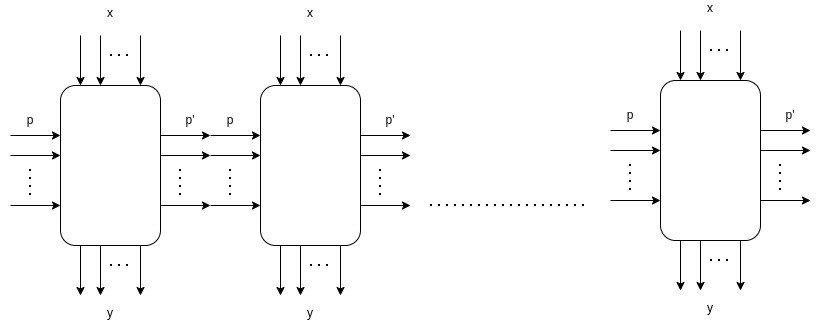
\includegraphics[width=0.8\textwidth]{img/diagram_iteracyjne.jpg}
    \caption{Ogólny schemat układu iteracyjnego.}
\end{figure}

\subsubsection*{Przykład: konwersja BIN -> Grey}
Konwersja liczby binarnej do kodu greya jest opisana na początku dokumentu. Polega na wykonywaniu sumy modulo 2. Zwykły układ kombinacyjny musiałby mieć ilość wejść równą ilości bitów konwertowanej liczby (po jednym wejściu na każdą pozycję w liczbie). Konwertując liczbę 16-bitową musielibyśmy wykonać układ 16-wejściowy, więc również bardzo skomplikowany. Dodatkowo, chcąc zmienić ilość bitów wejściowych, musimy przeprojektować cały układ od nowa.

Podejście iteracyjne pozwala nam zrealizować ten problem algorytmicznie. Ponieważ problem zakłada przetwarzanie jednej liczby w inną, zastosujemy wariant układów iteracyjnych z wyjściami z każdego bloku, bez dekodera. Wariant układu należy dobrać pod potrzeby danego zadania. Najpierw należy zdefiniować ile nasz układ będzie miał wejść i wyjść. Przypatrzmy się algorytmowi, możemy na nim zaznaczyć bit wejściowy $x$ (aktualną cyfrę przetwarzanej liczby), bit przeniesienia $p$ (informacja, jaka cyfra była przetwarzana przez poprzedni blok), wyjście $y$ realizujący naszą sumę modulo 2 oraz wyjście $p\prime$, które będzie informacją przekazywaną do kolejnego bloku o tym, jaką cyfrę właśnie przetworzyliśmy.

\begin{figure}[H]
    \centering
    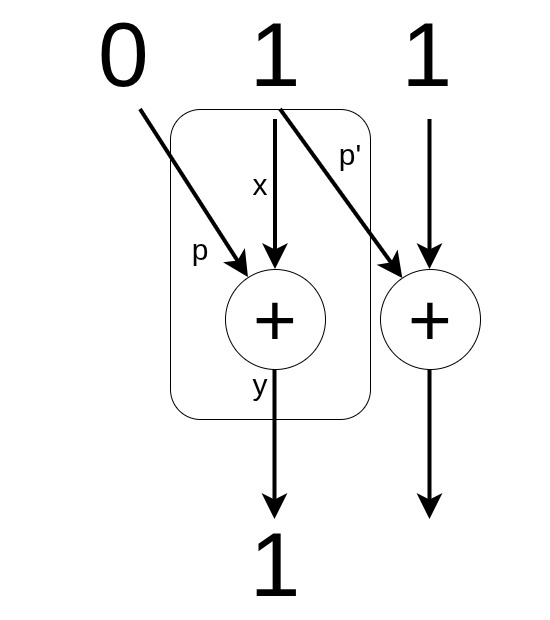
\includegraphics[width=0.4\textwidth]{img/bin_grey_converter.jpg}
    \caption{Schemat działania konwertera, zaznaczony pojedynczy blok z wejściami i wyjściami.}
\end{figure}

Skoro wiemy już jakie operacje będą wykonywane w bloku, zabieramy się za tabelę prawdy. Wyjście $y$ będzie rezultatem operacji sumy modulo 2 wejścia $p$ oraz $x$. Wyjście przeniesienia $p\prime$ przekazuje na kolejny blok wartość $x$, którą otrzymaliśmy w bloku aktualnym.

\begin{table}[h]
    \centering
    \begin{tabular}{|c|c|}
        $x$ $p$ & $y$ $p\prime$\\
        \hline
        0 0 & 0 0\\
        0 1 & 1 0\\
        1 1 & 0 1\\
        1 0 & 1 1\\
        \hline
    \end{tabular}
\end{table}

Na podstawie tej tabeli możemy narysować tabelę Karnaugh i wykonać minimalizację. Tabela po lewej przedstawia minimalizację wyjścia $y$, a tabela po prawej wyjścia $p\prime$.

\begin{center}
    \begin{karnaugh-map}[2][2][1][$p$][$x$]
    \minterms{1,2}
    \autoterms[0]
    \implicant{1}{1}
    \implicant{2}{2}
    \end{karnaugh-map}
    \begin{karnaugh-map}[2][2][1][$p$][$x$]
    \minterms{2,3}
    \autoterms[0]
    \implicant{2}{3}
    \end{karnaugh-map}
\end{center}

Wykorzystując tabelę możemy określić równania na oba wyjścia:
\begin{center}
    $y = x\bar{p} + \bar{x}p$ - minimalna postać wyjścia każdego bloku \\
    $p\prime = x$ - minimalna postać przeniesienia
\end{center} 

Mamy więc już wszystko, czego potrzebujemy do skonstruowania jednego bloku układu iteracyjnego. Każdy kolejny blok będzie identyczny. Blok będzie wyglądał następująco:

\begin{figure}[H]
    \centering
    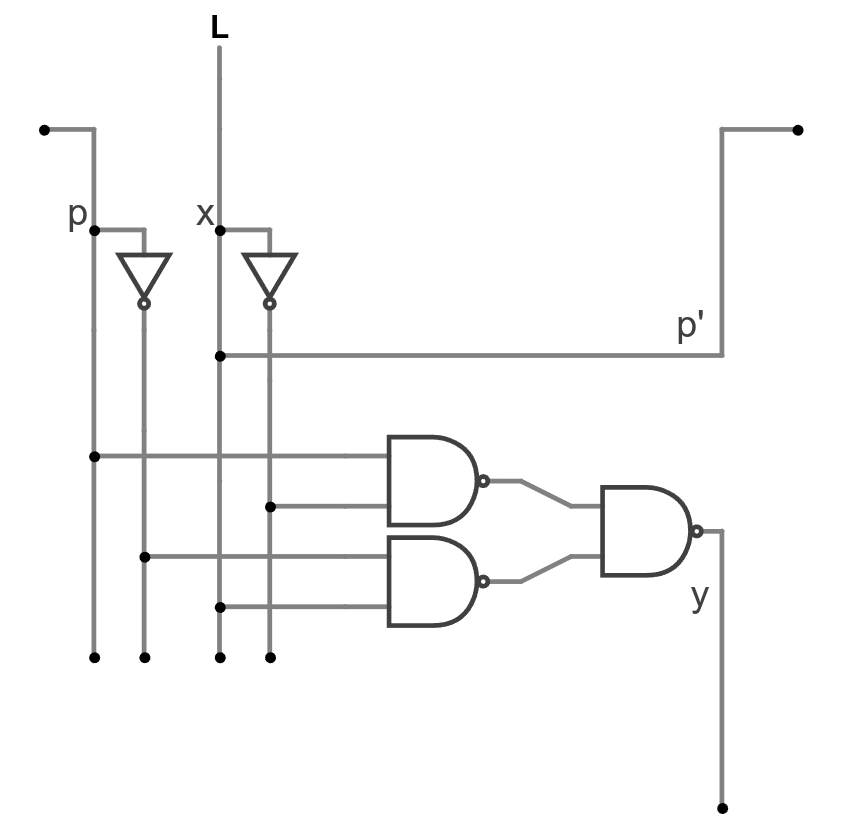
\includegraphics[width=0.7\textwidth]{img/bingrey_blok.png}
    \caption{Pojedynczy blok układu konwersji BIN -> Grey.}
\end{figure}

Na schemacie mamy wejście $p$ przeniesienia z poprzedniego bloku (którego na rysunku jeszcze nie ma), wejście $x$ na aktualny blok, wyjście $p\prime$, które jest przekazywane na wejście $p$ kolejnego bloku oraz wyjście $y$, na którym będzie prezentowana nasza liczba wyjściowa. Konwerter z jednym blokiem jest w stanie konwertować liczbę 1-bitową z binarnego do Greya, co nie jest wielkim wyczynem. Nasz układ pokaże swoje zalety dopiero w momencie połączenia ze sobą wielu (dowolnej ilości) bloków. Wykonajmy więc układ z czterema takimi blokami, aby konwertować liczbę 4-bitową.

\begin{figure}[H]
    \centering
    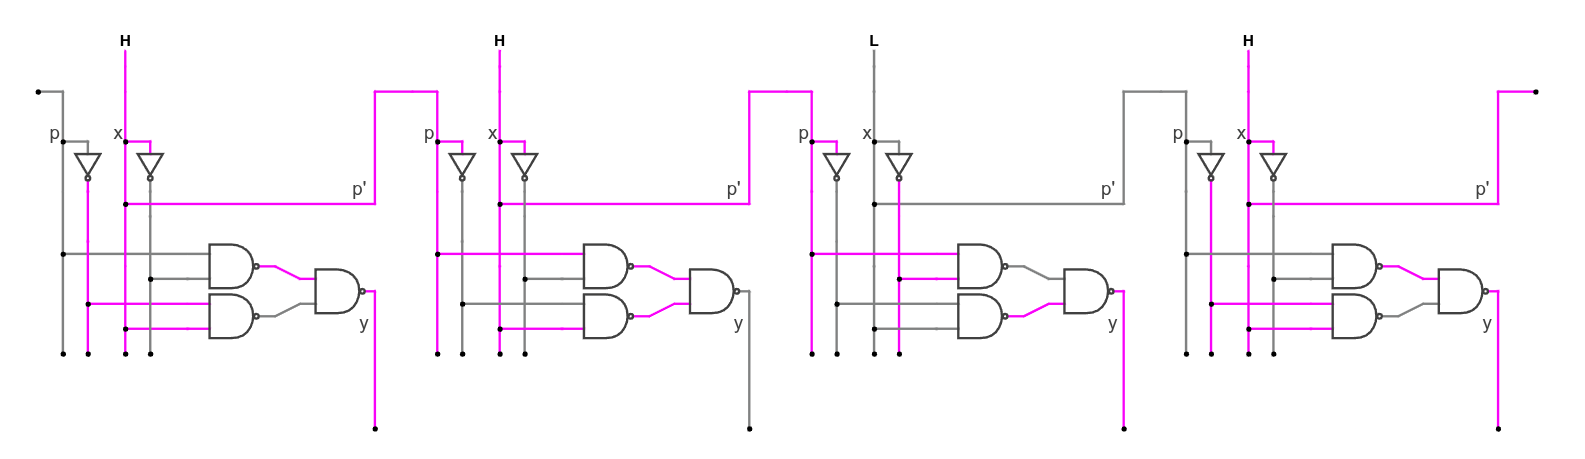
\includegraphics[width=1.0\textwidth]{img/bingrey_4bit.png}
    \caption{Układ 4-bitowej konwersji BIN -> Grey. Fioletowy przewód oznacza sygnał 1, szary 0.}
\end{figure}

Na rysunku widać cztery identyczne bloki. Warto zauważyć, że wejście $p$ pierwszego bloku od lewej jest niepodłączone. W zadaniu zawsze musimy określić \textbf{przeniesienie początkowe}, czyli stan, w którym znajduje się nasz układ na początku łańcucha bloków. Jest to kluczowe do poprawnej pracy układu. W naszym przypadku, patrząc na algorytm konwersji, stan początkowy przeniesienia powinien wynosić 0 i musimy to jasno zapisać przy rozwiązywaniu zadania. Na wejścia $x$ bloków podaliśmy liczbę 1101\textsubscript{2}. Na rysunku widać odpowiedzi bloków, których wyjścia przyjmują odpowiednie stany na podstawie wejść $x$ oraz $p$. Wyjście $p\prime$ jest połączone z wejściem $p$ kolejnego bloku. Na wyjściach $y$ powstaje nam liczba 1011\textsubscript{Grey}, czyli odpowiednik liczby wejściowej w kodzie Greya. Uzyskaliśmy więc układ konwertujący liczbę binarną do Greya, który możemy rozszerzyć do przetwarzania liczby o dowolnej liczbie bitów dodając jedynie więcej identycznych bloków do łańcucha.

\subsubsection*{Przykład: detekcja sekwencji}
Dostajemy zadanie: w ciągu dowolnej długości wykryć zadaną sekwencję. Przykładowo, wykrywamy sekwencję "1001". Oznacza to, że wyjście naszego układu ma wynosić 1, gdy w ciągu wejściowym (czyli w liczbie podawanej na wejścia naszych bloków, po bicie na blok) znajduje się dana sekwencja. W tego typu zadaniu zakładamy z reguły, że liczba bloków tworzących układ jest dowolna (zależy od długości ciągu, który chcemy sprawdzać). Z reguły też na każdy blok będzie podawany jeden bit z tego ciągu (ale wcale nie musi tak być). Ponieważ nasz układ ma zwracać informację, czy sekwencja w ogóle znajduje się w naszym ciągu, wykorzystamy typ układu z \textbf{dekoderem}. Dekoder będzie ostatnim blokiem naszego układu, który będzie odczytywał stan końcowy łańcucha bloków przed nim i na tej podstawie określał wartość wyjścia. Każdej kombinacji bitów przeniesienia będziemy więc nadawać wartość wyjścia $y$.

Pierwszym etapem zadania będzie określenie w jakich \textbf{stanach} nasz układ może się znajdować. Stany określamy sami na podstawie treści zadania. Pamiętajmy, że w każdym kolejnym bloku dostajemy kolejny bit ciągu wejściowego.